\documentclass[12pt]{article}
\usepackage[a4paper, left=2cm, right=2cm, top=2cm, bottom=2cm]{geometry}
\usepackage{dsfont}
\usepackage[fleqn]{amsmath}
\usepackage{amssymb,amstext}
\usepackage{graphicx}
\begin{document}
\setcounter{secnumdepth}{0}
\begin{center}
	UNIVERSIDADE FEDERAL DA PARAÍBA\\
	Probabilidade II\\
	Segunda Prova\\
	Paulo Ricardo Seganfredo Campana
\end{center}

\section{Questão 1.}

\[X \sim U \left( 0, \dfrac{1}{2} \right) \qquad Y = e^{2X}\]
\[S_{X} = \left( 0, \dfrac{1}{2} \right) \qquad S_{Y} = (e^{2 \cdot 0}, e^{2 \cdot \frac{1}{2}}) = (1, e)\]
\[F_{X}(x) = \dfrac{x-a}{b-a} = \dfrac{x}{\frac{1}{2}} = 2x \qquad a \leq x \leq b\]

\subsection{a)}

\[F_{Y}(y) = P(Y \leq y) = P(e^{2X} \leq y) = P(2X \leq \ln y) = P \left( X \leq \dfrac{\ln y}{2} \right) = F_{X} \left( \dfrac{\ln y}{2} \right)\]
\[F_{X} \left( \dfrac{\ln y}{2} \right) = 2\left( \dfrac{\ln y}{2} \right) = \ln y \longrightarrow F_{Y}(y) =
\left\{ \begin{array}{@{}l@{}}
	0 \qquad \text{se} \qquad y \leq 1, \\
	\ln y \quad \text{se } 1 \leq y \leq e, \\
	1 \qquad \text{se } e \leq y.  \\
\end{array} \right.\]
\[f_{Y}(y) = F_{Y}'(y) = (\ln y)' = \dfrac{1}{y} \longrightarrow f_{Y}(y) =
\left\{ \begin{array}{@{}l@{}}
	0 \qquad \text{se} \qquad y \leq 1, \\
	\dfrac{1}{y} \hspace{+21pt} \text{se } 1 \leq y \leq e, \\
	0 \qquad \text{se } e \leq y.  \\
\end{array} \right.\]

\begin{figure}[h!]
	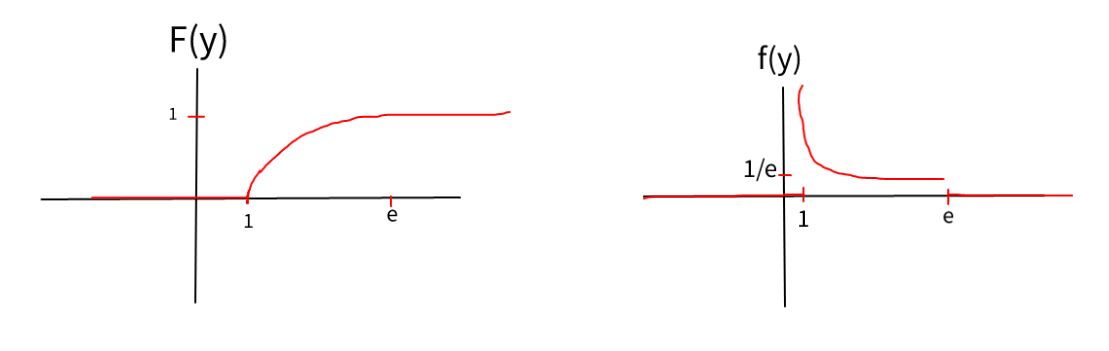
\includegraphics[scale=0.45]{q1}
\end{figure}

\subsection{b)}

\[E(Y) = \int_{1}^{e} y \dfrac{1}{y} dy = \int_{1}^{e} 1 dy = y \biggr|^{e}_{1} = e-1\]
\[E(Y^{2}) = \int_{1}^{e} y^{2} \dfrac{1}{y} dy = \int_{1}^{e} y dy = \dfrac{y^{2}}{2} \biggr|^{e}_{1} = \dfrac{e^{2}-1}{2}\]
\[Var(Y) = \dfrac{e^{2}-1}{2} - (e-1^{2}) = \dfrac{e^{2}-1}{2} - \dfrac{2e^{2}-4e+2}{2} = \dfrac{-e^{2}+4e-3}{2} = -\dfrac{1}{2}(e-1)(e-3)\]

\section{Questão 2.}

\[X \sim Exp(\lambda) \qquad Y = aX+b\]
\[E(X) = \dfrac{1}{\lambda} \qquad Var(X) = \dfrac{1}{\lambda^{2}} \qquad M_{X}(t) = \dfrac{\lambda}{\lambda-t}\]

\subsection{a)}

\[M_{Y}(t) = e^{bt}M_{X}(at) = e^{bt}\dfrac{\lambda}{\lambda-at} = \lambda (e^{bt} (\lambda-at)^{-1})\]

\subsection{b)}

\[M_{Y}'(t) = \lambda (e^{bt}(a)(\lambda-at)^{-2} + (\lambda-at)^{-1}be^{bt})\]
\[M_{Y}'(0) = \lambda (a\lambda^{-2} + \lambda^{-1}b) = \dfrac{a}{\lambda}+b = \dfrac{a+b\lambda}{\lambda}\]
\[M_{Y}''(t) = \lambda (a(e^{bt}(2a)(\lambda-at)^{-3}) + be^{bt}(\lambda-at)^{-2} + (\lambda-at)^{-1}b^{2}e^{bt} + (a)(\lambda-at)^{-2}be^{bt})\]
\[M_{Y}''(0) = \lambda(2a^{2}\lambda^{-3} + ab\lambda^{-2} + \lambda^{-1}b^{2} + a\lambda^{-2}b)\]
\[\hspace{+37pt} = \dfrac{2a^{2} + 2ab\lambda + b^{2}\lambda^{2}}{\lambda^{2}} = \dfrac{a^{2} + (a+b\lambda)^{2}}{\lambda^{2}}\]
\[Var(Y) = \dfrac{a^{2} + (a+b\lambda)^{2}}{\lambda^{2}} - \dfrac{(a+b\lambda)^{2}}{\lambda^{2}} = \dfrac{a^{2}}{\lambda^{2}}\]

\subsection{c)}

\[E(Y) = E(aX+b) = b+aE(X) = b+a\dfrac{1}{\lambda} = \dfrac{a+b\lambda}{\lambda}\]
\[Var(Y) = Var(aX+b) = a^{2}Var(X) = a^{2}\dfrac{1}{\lambda^{2}} = \dfrac{a^{2}}{\lambda^{2}}\]

\section{Questão 3.}

\[X \sim Exp(\lambda) \qquad \mu = E(X) = \dfrac{1}{\lambda} \qquad Var(X) = \dfrac{1}{\lambda^{2}}\]
Pela desigualdade clássica de Chebyshev:
\[P(|X-\mu| \geq \alpha) \leq \dfrac{1}{\alpha^{2}} Var(X)\]
\[P\left( \biggr| X-\dfrac{1}{\lambda} \biggr| \geq \alpha \right) \leq \dfrac{1}{\alpha^{2}\lambda^{2}}\]
Por serem eventos disjuntos, podemos separar $P(|X-\lambda| \geq \alpha)$ em duas probabilidades:
\[P\left( \biggr| X-\dfrac{1}{\lambda} \biggr| \geq \alpha \right) = P\left( X-\dfrac{1}{\lambda} \geq \alpha \right) + P\left( X-\dfrac{1}{\lambda} \leq -\alpha \right) =\]
\[P\left( X \geq \dfrac{1}{\lambda}+\alpha \right) + P\left( X \leq \dfrac{1}{\lambda}-\alpha \right)\]
$P\left( X \leq \dfrac{1}{\lambda}-\alpha \right)$ é positivo por ser uma probabilidade, portanto:
\[P\left( X \geq \dfrac{1}{\lambda}+\alpha \right) \leq P\left( \biggr| X-\dfrac{1}{\lambda} \biggr| \geq \alpha \right) \leq \dfrac{1}{\alpha^{2}\lambda^{2}}\]
Escolha $\alpha = \dfrac{2}{\lambda}$
\[P\left( X \geq \dfrac{3}{\lambda} \right) \leq P\left( \biggr| X-\dfrac{1}{\lambda} \biggr| \geq \alpha \right) \leq \dfrac{1}{4}\]
\[P\left( X \geq \dfrac{3}{\lambda} \right) \leq \dfrac{1}{4}\]




















\end{document}